\newif\iflinenumbers
% Comment in: 
\linenumberstrue  % want line numbers
% \linenumbersfalse % want no line numbers

% TODO Clean this up

\documentclass[12pt,oneside,notitlepage,abstracton,a4paper]{article}


% TODO: Find out what these are for
\usepackage{epsfig,scrpage2}
\usepackage{amsmath}
\usepackage{makecell}
\usepackage{graphicx}
\usepackage{booktabs}
\usepackage{arydshln}
\usepackage{setspace} % For singlespace
\usepackage[utf8]{inputenc}
\usepackage[T1]{fontenc}


%%%%%%%%%%%%%%%%%%%%%%%%%%%%%%%%%%%%%%%%%%%%%%%%%%%%%%%%%%%%%%%%%%%%%%%%%%%%%%%%
% Document layout
%%%%%%%%%%%%%%%%%%%%%%%%%%%%%%%%%%%%%%%%%%%%%%%%%%%%%%%%%%%%%%%%%%%%%%%%%%%%%%%%
% TODO Put some order into this part

% For Titlepage
\renewcommand{\headfont}{\normalfont}
  % \cfoot{\pagemark}
  \date{\normalsize \today}
\newcommand{\hwidthline}{
  \noindent\makebox[\linewidth]{\rule{\linewidth}{0.4pt}}
}
%-------------------------------------------------------------------------------
% For TODOS:
\newenvironment{TODOlist}{%
    \begin{list}{\textcolor{DESYorange}{!}\textcolor{DESYcyan}{$\bullet$}\textcolor{DESYorange}{!}}{\setlength{\itemsep}{0.5pt}}
  }{%
    \end{list}%
}

%-------------------------------------------------------------------------------
% To avoid float-only pages change minimum content on page that is necessary 
% for page to become float-only
\renewcommand{\floatpagefraction}{.7}

%-------------------------------------------------------------------------------
% For manipulating counters (e.g. figure counter in appendix)
\usepackage{chngcntr}

%-------------------------------------------------------------------------------
% In appendix use the section letter as first numbering letter for everything
\newcommand{\setappendixnumbering}{%
  \renewcommand{\thesection}{\Alph{section}}
  \renewcommand{\theequation}{\thesection.\arabic{equation}}
  \renewcommand{\thefigure}{\thesection.\arabic{figure}}
  \renewcommand{\thetable}{\thesection.\arabic{table}}
  \counterwithin{equation}{section}
  \counterwithin{figure}{section}
  \counterwithin{table}{section}
}

%-------------------------------------------------------------------------------
% Never break footnote onto multiple pages!
\interfootnotelinepenalty=10000

%-------------------------------------------------------------------------------
% Prevent floats to appear below footnotes
\usepackage[bottom]{footmisc}

%-------------------------------------------------------------------------------
% Remove section numbering
% \makeatletter
%   \renewcommand\@seccntformat[1]{}
% \makeatother

%-------------------------------------------------------------------------------
% Add line numbering
\iflinenumbers
  \usepackage{lineno}
  \linenumbers
\fi

%-------------------------------------------------------------------------------
% For affiliations
\usepackage[affil-it]{authblk}

%-------------------------------------------------------------------------------
% Title page layout (title, authors, affil)
\usepackage{etoolbox} % Tool to modify things (not sure, also need to sort somewhere better...)
\makeatletter % Change Title
\patchcmd{\@maketitle}{\LARGE \@title}{\fontsize{16}{19.2}\selectfont\@title}{}{}
\makeatother
\renewcommand\Authfont{\fontsize{12}{14.4}\selectfont}  % Change author
\renewcommand\Affilfont{\fontsize{9}{10.8}\itshape}     % Change affiliation

%-------------------------------------------------------------------------------
% Smaller side margins
\usepackage{geometry}
\geometry{
 total={170mm,257mm},
 left=20mm,
 top=20mm,
 }

%%%%%%%%%%%%%%%%%%%%%%%%%%%%%%%%%%%%%%%%%%%%%%%%%%%%%%%%%%%%%%%%%%%%%%%%%%%%%%%%
% Directory setup
%%%%%%%%%%%%%%%%%%%%%%%%%%%%%%%%%%%%%%%%%%%%%%%%%%%%%%%%%%%%%%%%%%%%%%%%%%%%%%%%

% Custom paths
\newcommand{\imagepath}{../Plots}
\newcommand{\logopath}{../Logos}
\newcommand{\feynmanpath}{./FeynmanDiagrams}


%%%%%%%%%%%%%%%%%%%%%%%%%%%%%%%%%%%%%%%%%%%%%%%%%%%%%%%%%%%%%%%%%%%%%%%%%%%%%%%%
% Graphics, Figures, Tables
%%%%%%%%%%%%%%%%%%%%%%%%%%%%%%%%%%%%%%%%%%%%%%%%%%%%%%%%%%%%%%%%%%%%%%%%%%%%%%%%

% Custom colors
\usepackage{xcolor}
\definecolor{DESYcyan}{RGB}{0,166,235}
\definecolor{DESYorange}{RGB}{242,142,0}
\definecolor{DESYgray}{RGB}{119,119,119}
\definecolor{bjetpurple}{RGB}{117,112,179}

%-------------------------------------------------------------------------------
% Feynman and other diagrams
\usepackage[compat=1.1.0]{tikz-feynman}
\usepackage{contour}
\usetikzlibrary{arrows,shapes,positioning}
\usetikzlibrary{decorations.markings}
\usetikzlibrary{decorations.pathmorphing}
\usetikzlibrary{decorations.pathreplacing}
\usetikzlibrary{patterns}
\usetikzlibrary{plotmarks}
\usetikzlibrary{shadows}

%-------------------------------------------------------------------------------
% Pretty captions and subcaptions
\usepackage[margin=8mm,font=small,labelfont=bf,format=plain]{caption}
\usepackage[margin=8mm,font=small,labelfont=bf,format=plain]{subcaption}

%-------------------------------------------------------------------------------
% Table top captions and alignment
\captionsetup[table]{position=top}
\captionsetup[subtable]{position=top}

%-------------------------------------------------------------------------------
% Nice features for tables
\usepackage{multirow} % Cells that span multiple rows
\newcommand{\vcell}[3]{\parbox[t]{#1}{\multirow{#2}{*}{\rotatebox[origin=c]{90}{#3}}}}

%-------------------------------------------------------------------------------
% Allows fixing float positions with the [H] option
% \usepackage{float}

%-------------------------------------------------------------------------------
% Shortcut for referencing a subfigure within a figure caption
\newcommand{\subfigref}[1]{({\protect\subref{#1}})}

%-------------------------------------------------------------------------------
% Force floats to appear in its section
% \usepackage[section]{placeins}

%%%%%%%%%%%%%%%%%%%%%%%%%%%%%%%%%%%%%%%%%%%%%%%%%%%%%%%%%%%%%%%%%%%%%%%%%%%%%%%%
% Text manipulation
%%%%%%%%%%%%%%%%%%%%%%%%%%%%%%%%%%%%%%%%%%%%%%%%%%%%%%%%%%%%%%%%%%%%%%%%%%%%%%%%

% Hyperlinks in pdf
\usepackage[
  bookmarks,                   %% PDF-Lesezeichen
  bookmarksopenlevel=1,        %% ...um eine Ebene
  bookmarksnumbered=true,      %% Lesezeichen numerieren
  pdfstartpage={1},            %% mit welcher Seite das PDF öffnen
  pdfstartview={FitH},         %% Zoom auf Seitenbreite
  pdfkeywords={},              %% Stichwörter fürs PDF, kommagetrennt
  pdfsubject={},               %% Themenbeschreibung kurz
  pdfcreator={LaTeX with KOMA-Script and hyperref package},
  hyperfootnotes=true,         %% Links auf Fußnoten
  linkbordercolor={0 1 1},     %% Rahmenfarbe interne Links
  menubordercolor={0 1 1},     %% Rahmenfarbe Literaturlinks
  urlbordercolor={1 0 0}       %% Rahmenfarbe externe Links
]{hyperref}                    %% Hyperlinks und Lesezeichen in PDF



%%%%%%%%%%%%%%%%%%%%%%%%%%%%%%%%%%%%%%%%%%%%%%%%%%%%%%%%%%%%%%%%%%%%%%%%%%%%%%%%
% Additions for math
%%%%%%%%%%%%%%%%%%%%%%%%%%%%%%%%%%%%%%%%%%%%%%%%%%%%%%%%%%%%%%%%%%%%%%%%%%%%%%%%

% Symbols with text above/below
\newcommand{\textover}[2]{\stackrel{\text{#2}}{#1}}
\newcommand{\eqtext}[1]{\textover{=}{#1}} %Equal sign with text over it

%-------------------------------------------------------------------------------
% Dirac notation
\usepackage{slashed}

%-------------------------------------------------------------------------------
% New fancy command for column vector with any number of rows
% (Taken from https://tex.stackexchange.com/questions/2705/typesetting-column-vector)
\newcount\colveccount
\newcommand*\colvec[1]{
        \global\colveccount#1
        \begin{pmatrix}
        \colvecnext
}
\def\colvecnext#1{
        #1
        \global\advance\colveccount-1
        \ifnum\colveccount>0
                \\
                \expandafter\colvecnext
        \else
                \end{pmatrix}
        \fi
}

%%%%%%%%%%%%%%%%%%%%%%%%%%%%%%%%%%%%%%%%%%%%%%%%%%%%%%%%%%%%%%%%%%%%%%%%%%%%%%%%
% Code
%%%%%%%%%%%%%%%%%%%%%%%%%%%%%%%%%%%%%%%%%%%%%%%%%%%%%%%%%%%%%%%%%%%%%%%%%%%%%%%%
% For code snipplet inputs
\usepackage{lmodern}
\usepackage{listings}
\lstset{
  language=[90]Fortran,
  basicstyle=\footnotesize,        % the size of the fonts that are used for the code
  keywordstyle=\color{red},
  commentstyle=\color{green},
  morecomment=[l]{!\ }% Comment only with space after !
  breaklines=true,                 % sets automatic line breaking
  frame=single,	                   % adds a frame around the code
  keepspaces=true,                 % keeps spaces in text, useful for keeping indentation of code (possibly needs columns=flexible)
  % numbers=left,                    % where to put the line-numbers; possible values are (none, left, right)
  % numbersep=5pt,                   % how far the line-numbers are from the code
  % numberstyle=\tiny\color{mygray}, % the style that is used for the line-numbers
  % stepnumber=2,                    % the step between two line-numbers. If it's 1, each line will be numbered
  rulecolor=\color{black},         % if not set, the frame-color may be changed on line-breaks within not-black text (e.g. comments (green here))
  showspaces=false,                % show spaces everywhere adding particular underscores; it overrides 'showstringspaces'
  showstringspaces=false,          % underline spaces within strings only
  showtabs=false,                  % show tabs within strings adding particular underscores
  % tabsize=2,	                   % sets default tabsize to 2 spaces
}


%%%%%%%%%%%%%%%%%%%%%%%%%%%%%%%%%%%%%%%%%%%%%%%%%%%%%%%%%%%%%%%%%%%%%%%%%%%%%%%%
% Bibliography
%%%%%%%%%%%%%%%%%%%%%%%%%%%%%%%%%%%%%%%%%%%%%%%%%%%%%%%%%%%%%%%%%%%%%%%%%%%%%%%%
\usepackage[english]{babel}% Recommended
\usepackage{csquotes}% Recommended
\usepackage[style=numeric-comp,sorting=none]{biblatex}
\addbibresource{library.bib}% Syntax for version >= 1.2

\newcommand{\customprintbibliography}{%
  % \begingroup
  \printbibliography[heading=none]
  % \endgroup
  \newpage
}


%%%%%%%%%%%%%%%%%%%%%%%%%%%%%%%%%%%%%%%%%%%%%%%%%%%%%%%%%%%%%%%%%%%%%%%%%%%%%%%%
% Symbol shortcuts
%%%%%%%%%%%%%%%%%%%%%%%%%%%%%%%%%%%%%%%%%%%%%%%%%%%%%%%%%%%%%%%%%%%%%%%%%%%%%%%%

\usepackage{amssymb}

%-------------------------------------------------------------------------------
% Math/physics symbols
\newcommand{\Lagr}{\mathcal{L}}
\newcommand{\mbar}{\bar{m}}
\newcommand{\oper}{\mathcal{O}}
\newcommand{\DEG}{^{\circ}}

%-------------------------------------------------------------------------------
% Line stuff
\newcommand{\flend}{&&\\} % End of a flalign newenvironment line

%-------------------------------------------------------------------------------
% Particles
\newcommand{\eP}{e^{+}}
\newcommand{\eM}{e^{-}}
\newcommand{\lP}{l^{+}}
\newcommand{\lM}{l^{-}}

\newcommand{\fbar}{\bar{f}}

\newcommand{\eL}{\eM_{L}}
\newcommand{\eR}{\eM_{R}}
\newcommand{\pL}{\eP_{L}}
\newcommand{\pR}{\eP_{R}}

\newcommand{\nue}{\nu_e}
\newcommand{\numu}{\nu_{\mu}}
\newcommand{\nutau}{\nu_{\tau}}
\newcommand{\nul}{\nu_l}

\newcommand{\nubar}{\bar{\nu}}
\newcommand{\nuebar}{\bar{\nue}}
\newcommand{\nulbar}{\bar{\nul}}

\newcommand{\qbar}{\bar{q}}
\newcommand{\qu}{q_{u}}
\newcommand{\qd}{q_{d}}
\newcommand{\qubar}{\bar{q}_{u}}
\newcommand{\qdbar}{\bar{q}_{d}}

\newcommand{\tbar}{\bar{t}}

\newcommand{\vis}{\text{vis}}
\newcommand{\inv}{\text{inv}}

\newcommand{\WP}{W^{+}}
\newcommand{\WM}{W^{-}}

%%%%%%%%%%%%%%%%%%%%%%%%%%%%%%%%%%%%%%%%%%%%%%%%%%%%%%%%%%%%%%%%%%%%%%%%%%%%%%%%
%%%%%%%%%%%%%%%%%%%%%%%%%%%%%%%%%%%%%%%%%%%%%%%%%%%%%%%%%%%%%%%%%%%%%%%%%%%%%%%%










%TODO TO ORDER:
%%%%%%%%%%%%%%%%%%%%%%%%%%%%%%%%%%%%%%%%%%%%%%%%%%%%%%%%%%%%%%%%%%%%%%%%%%%%%%%%

% TODO What is this??
\setcounter{secnumdepth}{3}

\setlength{\parindent}{0em}
\setlength{\parskip}{0ex plus0.5ex minus0ex}
\pagestyle{scrheadings}

 

%^^^^^^^^^^^^^^^^^^^^^^^^^^^^^^^^^^^^^^^^^^^^^^^^^^^^^^^^^^^^^^^^^^^^^^^^^^^^^^^
% TODO For library execute: chmod u+x combine_bib_entries.sh && ./combine_bib_entries.sh

\begin{document}


%===============================================================================

% Titelpageseite
\begin{titlepage}

  \begin{center}
    
\includegraphics[height=3cm]{\logopath/DESY-logo}
  \end{center}

  \vspace{0em}

  \begin{minipage}[t]{\textwidth}

    \begin{minipage}{\linewidth}

      \vspace{0em}

      \begin{center}\bfseries\huge
        Doing cool things at the future\\ International Linear Collider
      \end{center}

      \vspace{1.0 em}

      \begin{center}\large
        Max Musterstudent\\
        University of Bielefeld\\
        Germany\\[0.5cm]
        September 5, 2019
      \end{center}

    \end{minipage}
  \end{minipage}
  
  \vspace{1cm}

  \begin{abstract}
    My cool abstract that makes every expert read this report.
  \end{abstract}

\end{titlepage}

\clearpage

%===============================================================================

\tableofcontents
\clearpage

%===============================================================================

\section{Introduction}
I am motivated to do my work and so should you be.

Here is what I will talk about in section~\ref{SEC:Main} and the rest.

%-------------------------------------------------------------------------------

\section{Example main text section}\label{SEC:Main}
Previous studies have shown that I can cite stuff~\cite{Fleper:2016frz}.

Plotting things makes them visual (see fig.~\ref{FIG:MassPlotsIDRL}).

\begin{figure}
  \centering
  \begin{subfigure}[t]{0.5\textwidth}
    \centering
    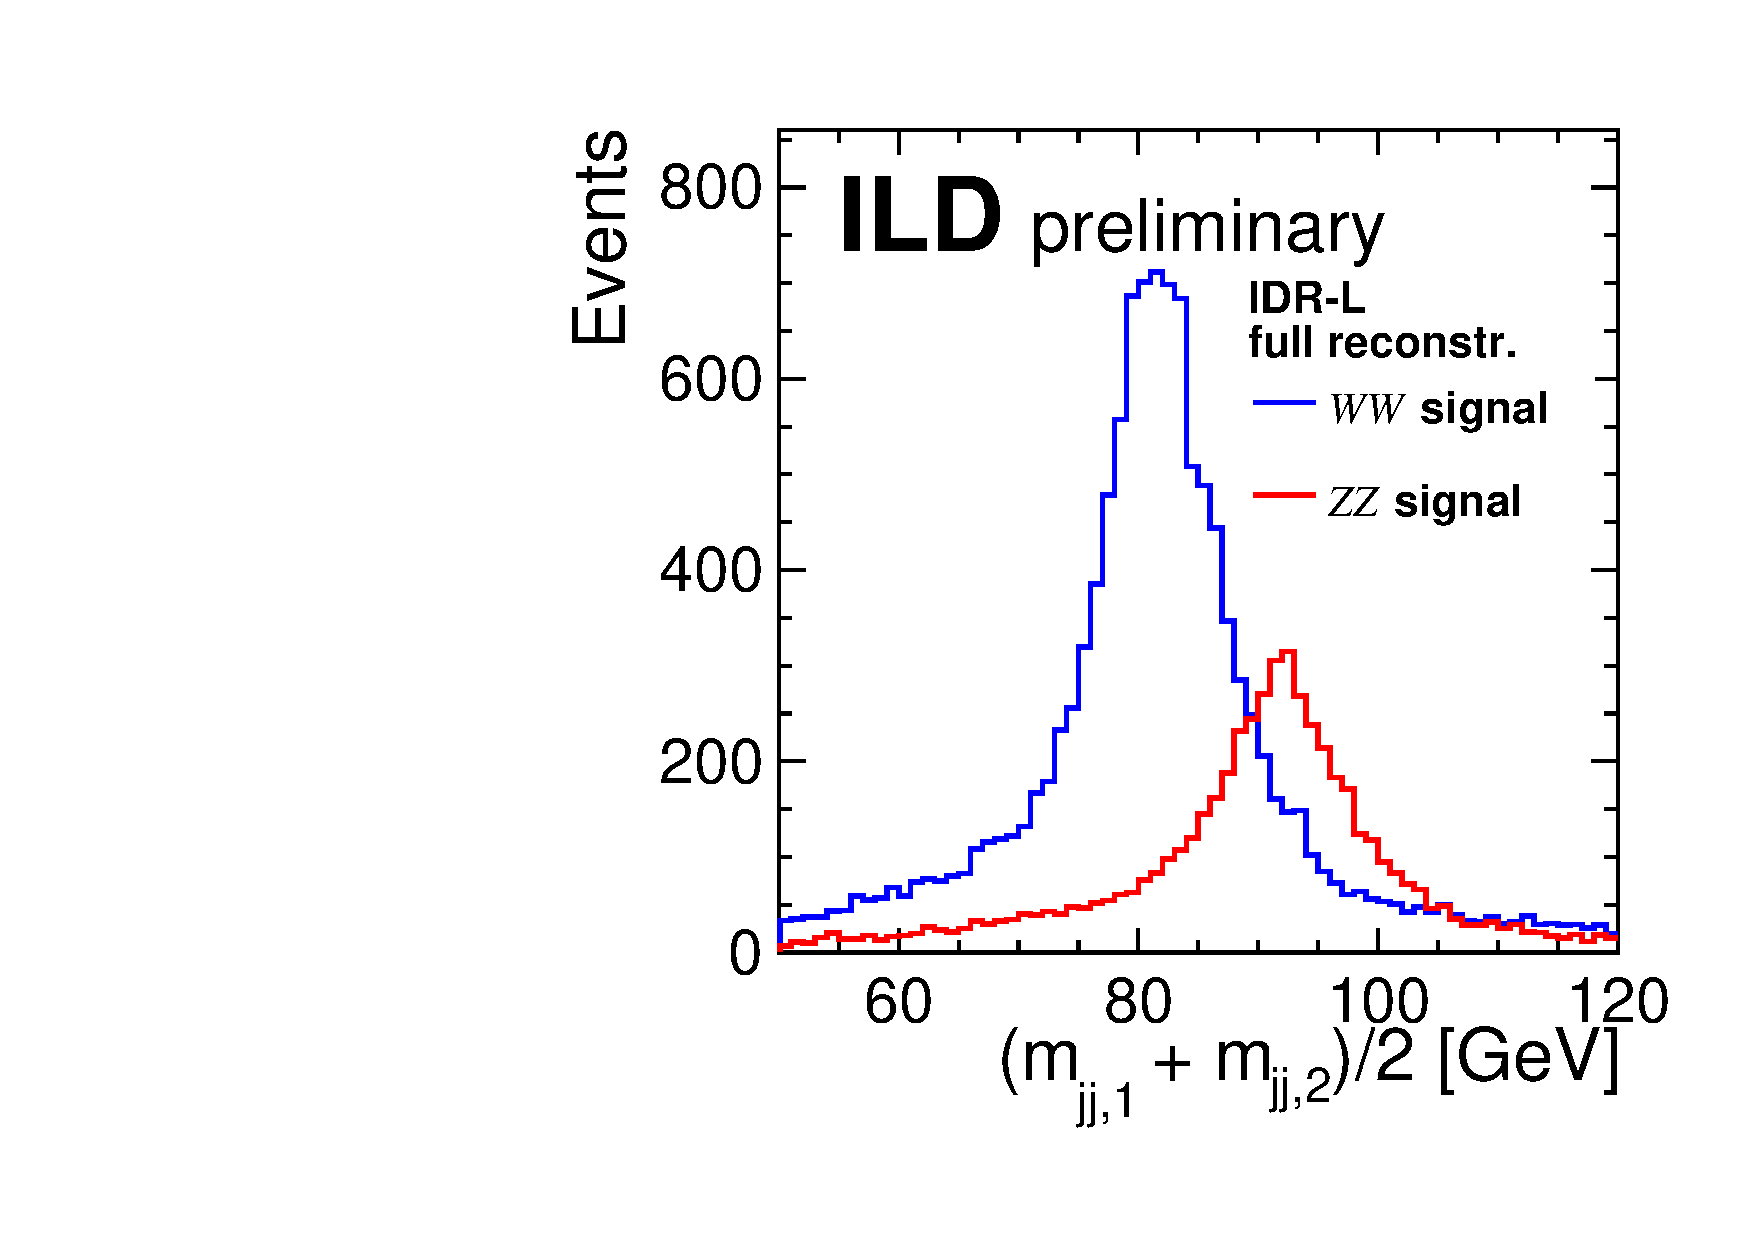
\includegraphics[width=\textwidth]{\imagepath/MassPlots/l5_m}
    \caption{}
    \label{SUBFIG:IDRL_m}
  \end{subfigure}%
  \begin{subfigure}[t]{0.5\textwidth}
    \centering
    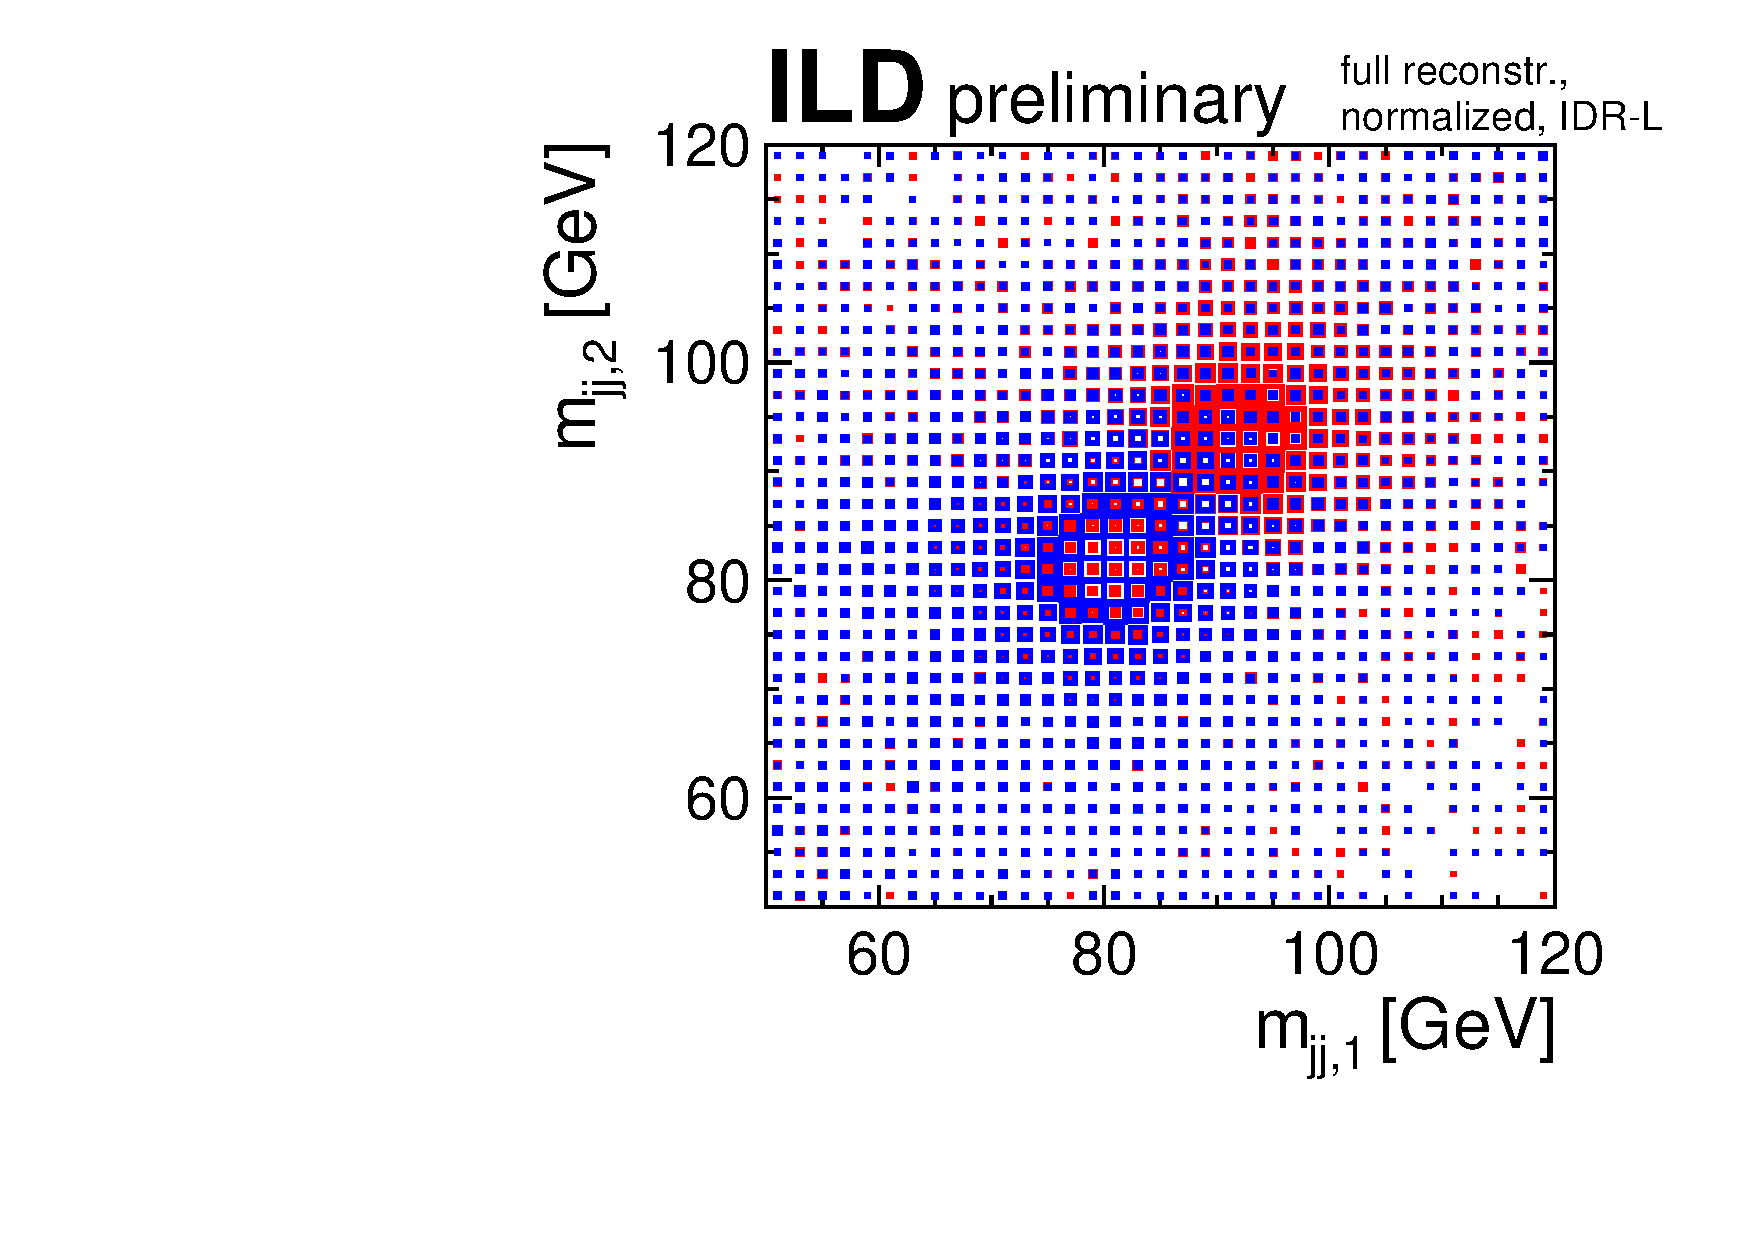
\includegraphics[width=\textwidth]{\imagepath/MassPlots/m_m_rec}
    \caption{}
    \label{SUBFIG:IDRL_m_m}
  \end{subfigure}
  \caption{
    Cool plots.
    \subfigref{SUBFIG:IDRL_m} This one is nice. 
    \subfigref{SUBFIG:IDRL_m_m} But this one is also nice.
  }
  \label{FIG:MassPlotsIDRL}
\end{figure}

In contrast, tables can sometimes be a bit dense and should be used with caution (see tab.~\ref{TAB:WWZZSeparationEfficiencies}).

\begin{table}
  \centering
  \caption{
    A table that shows numbers.
  } 
  \label{TAB:WWZZSeparationEfficiencies}
  \begin{tabular}{|l|l|l|l|l|} \hline
    Level & \multicolumn{4}{c|}{$\epsilon_{WW/ZZ} [\%]$} \\ \cline{2-5}
     & \multicolumn{2}{c|}{full $m_{VV}$ range} & \multicolumn{2}{c|}{$m_{VV}>500\,$GeV} \\ \cline{2-5}
     & IDR-L & IDR-S & IDR-L & IDR-S \\ \hline \hline
    Full reconstruction  & 71.1 & 71.5 & 73.0 & 72.9 \\ \hline
    Cheated overlay & 79.6 & 79.4 & 84.6 & 84.0 \\ \hline
    Cheated jets & 86.3 & 85.9 & 86.2 & 85.6 \\ \hline
    Cheated bosons & 88.4 & 88.1 & 86.6 & 86.1 \\ \hline
    No semi-leptonic events & 94.4 & 94.3 & 92.6 & 92.5 \\ \hline
  \end{tabular}
\end{table}

It is trivial that equations are important in physics so one could write one like this

\begin{equation} \label{EQ:ExactNeutrinoSolution}
  p_{\nu,\parallel} = \frac{1}{2 \cdot D} \cdot \left(-A \, \pm\, \sqrt{A^2 - BD} \right) \, 
\end{equation}

and describe all its symbols.

And one can even write many aligned ones

 \begin{align}
  A & =p_{\text{vis},\parallel} \cdot ( 2 p_{\text{vis},\perp}^2 + m_{\text{vis}}^2 - m_{X}^2) \\
  B & =4 p_{\text{vis},\perp}^2 \cdot E_{\text{vis}}^2 - ( 2 p_{\text{vis},\perp}^2 + m_{\text{vis}}^2 - m_{X}^2 )^2 \\
  D & =E_{\text{vis}}^2- p_{\text{vis},\parallel}^2
\end{align}

and also remember to describe all symbols used!

Sometimes it can be helpful for long formulas and $\eP\eM$ collisions to define shortcuts (see end of \texttt{Preamble.tex}).

If Feynman-diagrams are necessary (they are) then one can even do that (see fig.~\ref{FEY:SignalProcess}).

\begin{figure} 
  \centering
  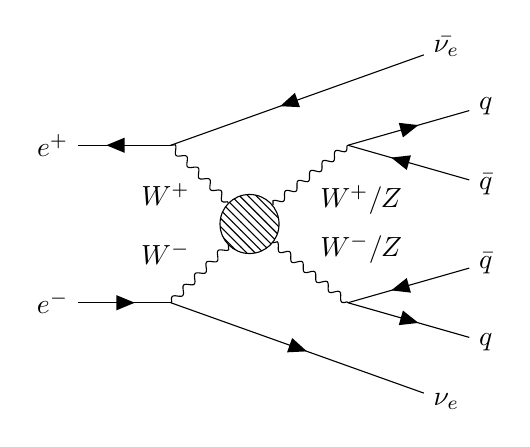
\begin{tikzpicture}
  \begin{feynman}[scale=1] % using the vertex in brackets () allows fixing of vertex
    \vertex[blob] (m) at (0, 0) {\contour{white}{}};
    \vertex (a) at (-1,-1);
    \vertex (b) at ( 1.25,-1) ;
    \vertex (c) at (-1, 1);
    \vertex (d) at ( 1.25, 1) ;
    \vertex (q1) at ( 3,-1.5) {$q$};
    \vertex (q2) at ( 3,-0.5) {$\bar{q}$};
    \vertex (q3) at ( 3, 1.5) {$q$};
    \vertex (q4) at ( 3, 0.5) {$\bar{q}$};
    \vertex (i1) at (-2.5,-1) {$e^-$};
    \vertex (o1) at ( 2.5,-2.25) {$\nu_e$};
    \vertex (i2) at (-2.5, 1) {$e^+$};
    \vertex (o2) at ( 2.5, 2.25) {$\bar{\nu_e}$};
    \diagram* {
      (i1) -- [fermion] (a) -- [fermion] (o1) ,
      (i2) -- [anti fermion] (c) -- [anti fermion] (o2) ,
      (a) -- [photon, edge label=$W^-$] (m),
      (m) -- [photon, edge label=$W^+$] (c),
      (b) -- [photon, edge label=$W^-/Z$, swap] (m),
      (d) -- [photon, edge label=$W^+/Z$] (m),
      (b) -- [fermion] (q1),
      (b) -- [anti fermion] (q2),
      (d) -- [fermion] (q3),
      (d) -- [anti fermion] (q4),
    };
  \end{feynman}
\end{tikzpicture}
  \caption{Pseudo Feynman diagram of vector boson scattering in the $\nu\nubar q\qbar q\qbar$ final state at $\eP\eM$ colliders.}
  \label{FEY:SignalProcess}
\end{figure}

%-------------------------------------------------------------------------------

\section{Conclusion}
We know some stuff and that is cool.
But we want to know more stuff.

So I had this idea to figure something new out.
I did it in a cool way.
And got some crazy results.

Now we know more about the thing.
And that can potentially be relevant at some point in human history.



%-------------------------------------------------------------------------------

\clearpage

\section{References}
\customprintbibliography

%-------------------------------------------------------------------------------

\clearpage
\section{Acknowledgments}
Special shout-out to coffee!

%===============================================================================

\clearpage

%-------------------------------------------------------------------------------

\section{Appendix}
\subsection{Potentially interesting details}

For plots, figures and calculation that:
\begin{itemize}
  \item are too detailed for main text
  \item are side remarks
  \item are slightly different versions of plots shown in the main text (but not different enough to need to be there)
  \item coooooouuuuuld be interesting if someone tries to repeat my study...
\end{itemize}


%===============================================================================

\end{document}

%_______________________________________________________________________________
